
\chapter{Introduction}
% \addcontentsline{toc}{chapter}{Introduction}

Artificial Intelligence (AI) and Machine Learning (ML) have emerged as transformative technologies across a wide range of engineering domains, enabling systems to learn complex patterns directly from data. Unlike traditional rule-based approaches, ML models can approximate highly nonlinear relationships without requiring explicit analytical formulations. This capability has made AI particularly powerful in domains characterized by high complexity, multi-physics interactions, and large-scale data, such as autonomous systems, robotics, and automotive engineering. In recent years, the integration of AI into automotive systems has accelerated significantly, supporting applications ranging from perception and control to energy management and predictive modeling.

Within the automotive domain, electric vehicles (EVs) present a particularly challenging environment due to their reliance on battery-driven energy systems and tightly coupled thermal dynamics. The battery serves as the primary power source not only for propulsion but also for auxiliary systems such as heating, ventilation, and air conditioning (HVAC). As a result, efficient thermal management becomes a critical requirement for ensuring both passenger comfort and system performance. The challenge becomes more pronounced under extreme environmental conditions. For instance, in cold climates where ambient temperatures may drop below $-20^\circ$C, or in hot regions where temperatures can exceed $50^\circ$C, the thermal system must regulate cabin conditions without imposing excessive load on the battery or degrading system efficiency.

A naive approach to thermal control, such as rapidly heating or cooling the cabin air to extreme temperatures, is neither energy-efficient nor comfortable for passengers. Instead, thermal systems must follow physically governed heat transfer processes, such as those described by Newton’s Law of Cooling, which states that the rate of temperature change is proportional to the difference between the system temperature and the ambient environment.

\begin{equation}
\frac{dT}{dt} = -k (T - T_{\text{env}})
\end{equation}

As a result, thermal behavior in EV systems is inherently dynamic and must be modeled over discrete time steps. Predicting this behavior requires capturing complex interactions between environmental conditions, system parameters, and energy constraints.
\\As illustrated in Fig.~\ref{fig:thermal_response}, the cabin temperature evolves gradually over time under both heating and cooling scenarios, reflecting the dynamic nature of thermal regulation.
\begin{figure}[H]
    \centering
    \includegraphics[width=0.85\textwidth]{figures/thermal_response.png}
    \caption{Illustration of Thermal response of cabin temperature over time under heating and cooling conditions}
    \label{fig:thermal_response}
\end{figure}


\section{Motivation}

The growing adoption of electric vehicles has intensified the demand for efficient thermal management solutions, as energy efficiency directly impacts vehicle range, performance, and battery lifespan. In recent years, AI-driven approaches have gained significant attention in automotive engineering, particularly for predictive modeling and system optimization. Data-driven surrogate models have been explored as a promising alternative to traditional simulation methods, enabling a rapid approximation of the behavior of the system with reduced computational cost.

Several studies have demonstrated the potential of machine learning techniques in modeling thermal systems, including regression-based models, neural networks, and hybrid physics-informed approaches. These methods leverage simulation or experimental data to learn input-output relationships, allowing fast predictions once trained. In the context of electric vehicle thermal management, such approaches can support applications such as real-time control, design optimization, and sensitivity analysis.

\begin{figure}[H]
    \centering
    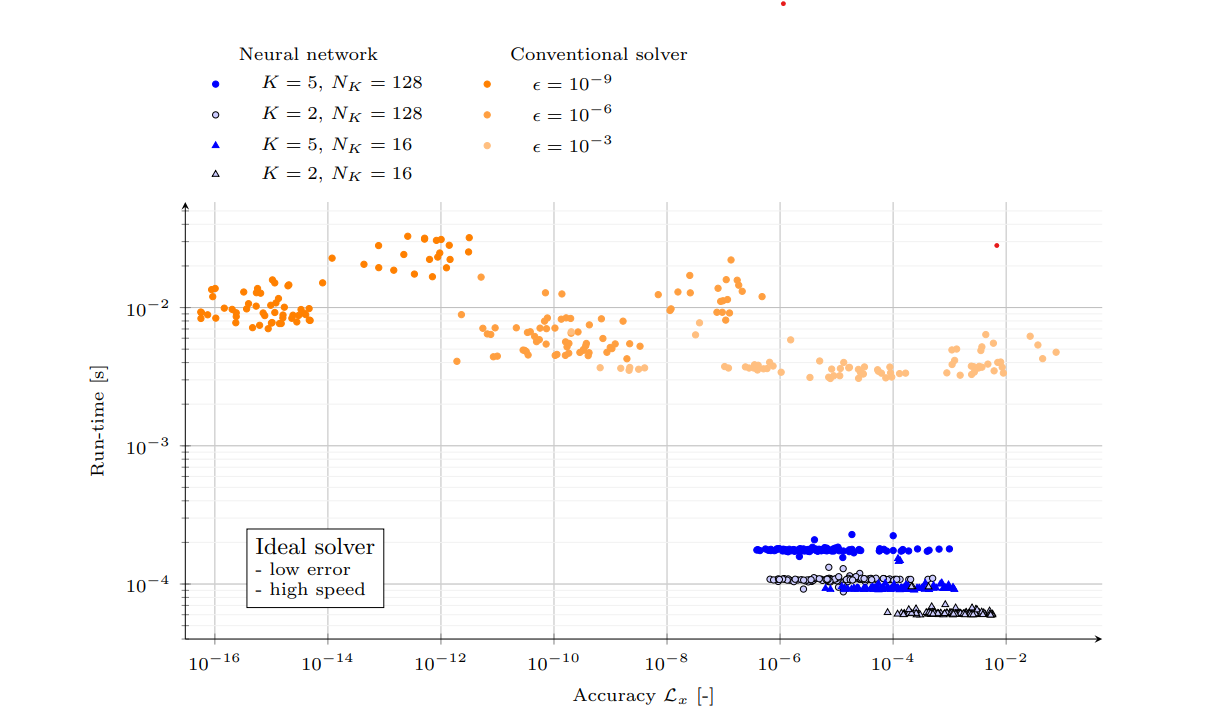
\includegraphics[width=0.85\textwidth]{figures/runtime_accuracy.png}
    \caption{Evaluation of run-time and accuracy for the 11-bus system under varying solver tolerances and neural network configurations. Reproduced from \cite{stiasny2023pinn}.}
    \label{fig:runtime_accuracy_tradeoff}
\end{figure}


Despite this progress, existing approaches face several limitations. Physics-based models, while accurate, remain computationally expensive and difficult to scale for large datasets or real-time deployment. However, purely data-driven models often struggle with high-dimensional outputs, particularly when dealing with time-series data representing dynamic system behavior. Additionally, efficient sampling of the input parameter space remains a challenge due to the curse of dimensionality, limiting the generalization capability of learned models.

To address these challenges, this thesis proposes a hybrid framework that combines high-fidelity physics-based simulations with machine learning techniques. By integrating efficient sampling strategies, dimensionality reduction, and surrogate modeling, the proposed approach aims to achieve a balance between computational efficiency and predictive accuracy. This enables scalable and real-time capable modeling of thermal systems in automotive applications.
% \begin{center}
%         \begin{minipage}[c]{0.6\textwidth}
%             \centering
%             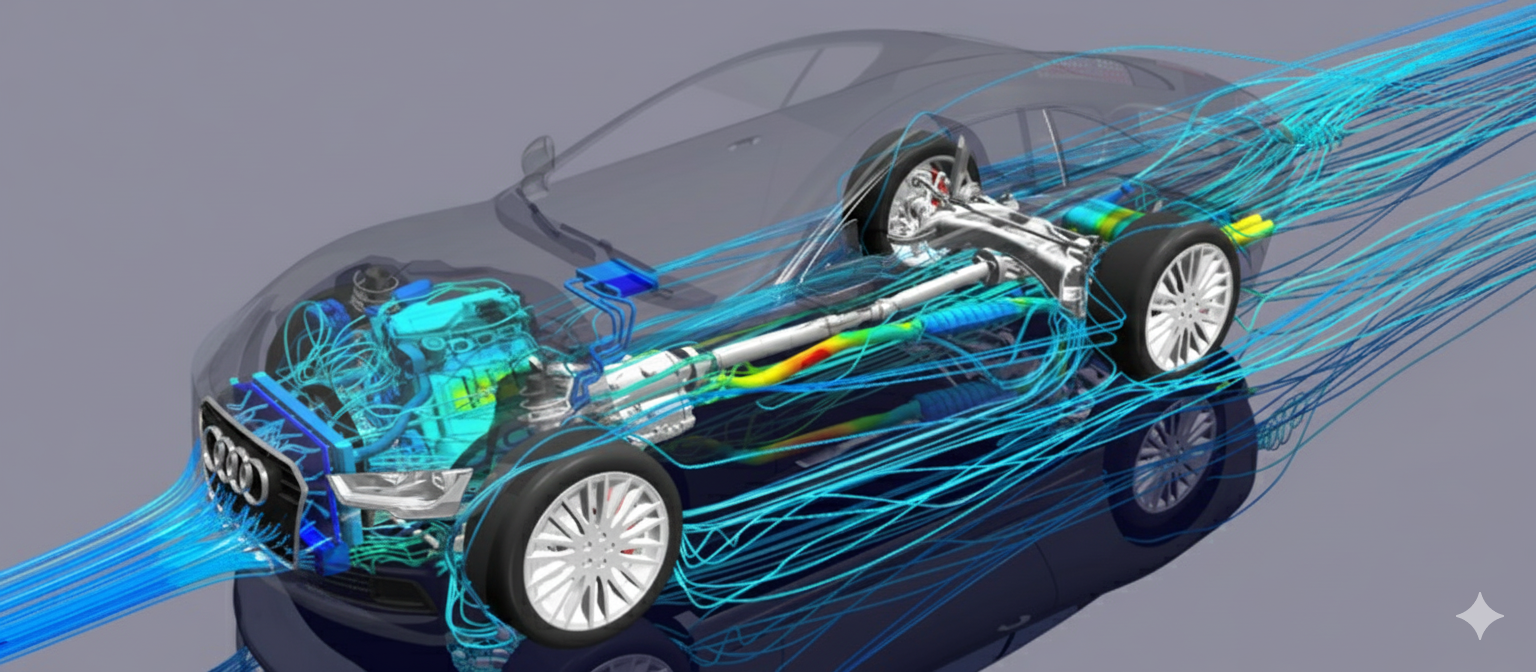
\includegraphics[width=\textwidth]{figures/Thermal_System_Audi.jpg}
%         \end{minipage}%
% \end{center} 
---

% \section{Contribution of this Thesis}

% This thesis presents a hybrid modeling framework that integrates physics-based simulation with machine learning to develop an efficient surrogate model for automotive thermal systems.

% The main contributions of this work are:

% \begin{itemize}
%     \item Development of a surrogate modeling pipeline based on high-fidelity Dymola simulations of an EV thermal management system.
%     \item Generation of a comprehensive dataset consisting of 2050 simulation runs using Latin Hypercube Sampling (LHS), covering diverse operating conditions including fast charging and race-track scenarios.
%     \item Application of Principal Component Analysis (PCA) to reduce the dimensionality of time-series outputs from 1800 time steps to a compact latent representation of 5 components while preserving more than 99% of the original variance.
%     \item Implementation of a Random Forest Regressor as a baseline model to learn the mapping from a 7-dimensional input space to the reduced latent output space.
%     \item Investigation of neural network–based approaches, including Multi-Layer Perceptron (MLP) models, to improve the representation of nonlinear and dynamic system behavior.
%     \item Reconstruction of full time-series outputs from the predicted latent space, enabling accurate and computationally efficient approximation of the original thermal system response.
% \end{itemize}
\begin{figure}[H]
    \centering
    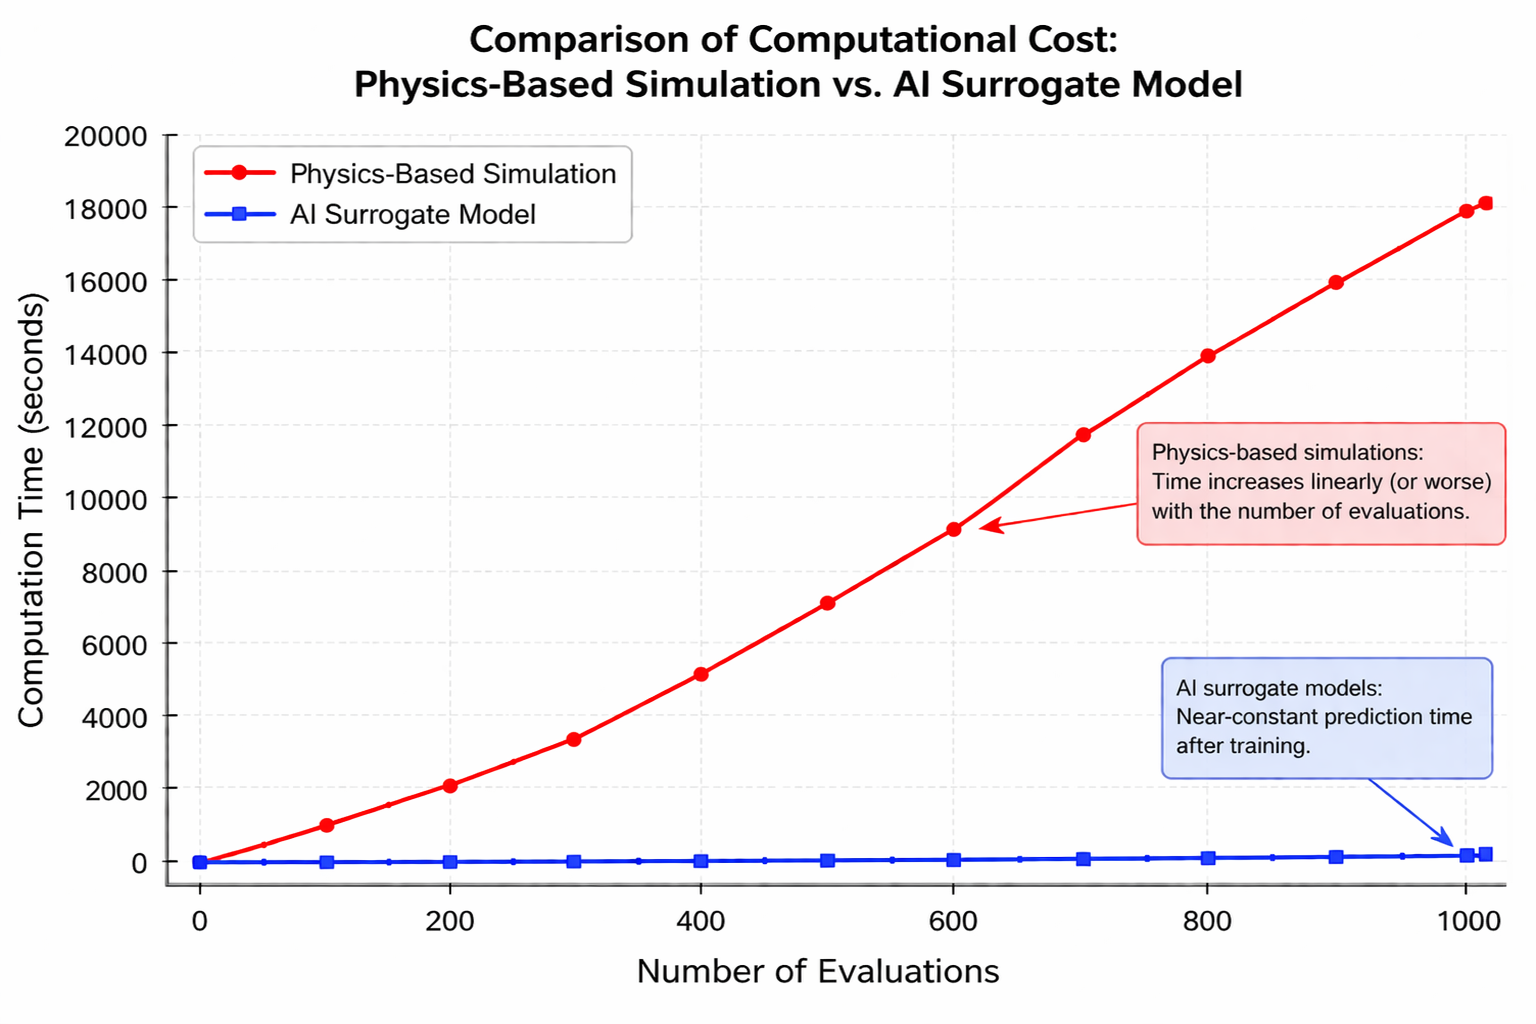
\includegraphics[width=0.85\textwidth]{figures/computational_cost.png}
    \caption{Comparison of computational cost between physics-based simulations and AI-based surrogate models. While simulation time increases with the number of evaluations, surrogate models provide near-constant inference time after training}
    \label{fig:simulation_vs_AI}
\end{figure}

\newpage

\section{Objectives}

The primary objective of this thesis is to develop a computationally efficient surrogate model capable of accurately predicting the thermal behavior of an automotive system under varying operating conditions.

The specific objectives are as follows.

\begin{itemize}
    \item To generate a representative dataset using Dymola simulations by varying operating conditions and boundary parameters across realistic automotive thermal scenarios.

    \item To efficiently explore the high-dimensional input space using Latin Hypercube Sampling while minimizing the number of required simulations.

    \item To reduce high-dimensional time-series outputs using PCA, enabling efficient learning while preserving essential thermal system dynamics.

    \item To develop and evaluate surrogate models, including Random Forest and MLP, for predicting thermal behavior from reduced latent representations.

    \item To compare prediction accuracy and computational efficiency of surrogate models against physics-based simulations using standard evaluation metrics.
\end{itemize}

% \begin{center}
%         \begin{minipage}[c]{0.6\textwidth}
%             \centering
%             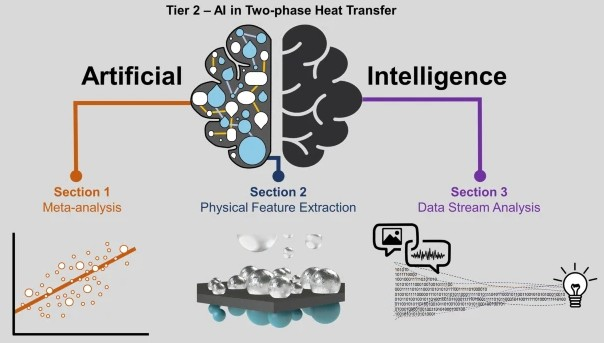
\includegraphics[width=\textwidth]{figures/AI_Thermal.jpg}
%         \end{minipage}%
% \end{center} 
% \newpage
---

\section{Structure of the Thesis}

This thesis is organized as follows:

\begin{itemize}
    \item Chapter 2 introduces the fundamental concepts related to thermal system modeling, machine learning, and dimensionality reduction techniques used in this work.
    \item Chapter 3 reviews existing literature on physics-based thermal modeling, sampling strategies, and surrogate modeling approaches.
    \item Chapter 4 presents the methodology, including data generation using Latin Hypercube Sampling, dimensionality reduction using PCA, and the development of machine learning models.
    \item Chapter 5 describes the experimental setup and evaluation framework.
    \item Chapter 6 presents and analyzes the results, comparing the performance of different surrogate models.
    \item Finally, Chapter 7 concludes the thesis and outlines potential directions for future work.
\end{itemize}


% \begin{center}
%         \begin{minipage}[c]{0.6\textwidth}
%             \centering
%             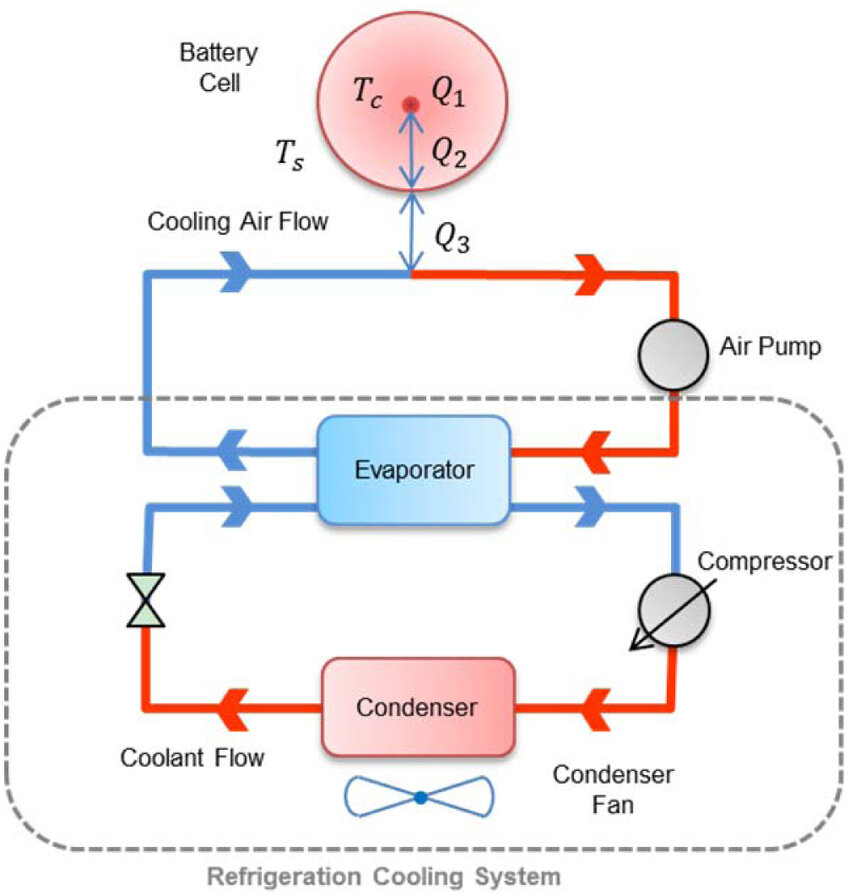
\includegraphics[width=\textwidth]{figures/Battery-thermal-management-system-structure-Q1-is-battery-heat-generation-Q2-and-Q3-are.png   }
%         \end{minipage}%
% \end{center}        
% \newpage
% ---




